\documentclass{article}
\usepackage{graphicx}


\usepackage[a4paper, total={6in, 8in}]{geometry}
\title{OOAD Project Phase 1: Hospital}
\author{Charles Treat}
\graphicspath{ {./images/} }
\begin{document}

\maketitle

\section{Methodologies for Information Gathering}
In order to best understand the internal processes of a hospital and the needs they serve, I utilized two different intial
information gathering methods to gain a foundational understanding. I first interviewed my sister, Jo Treat a former hospital nurse. Through
this interview, I was able to get a good grasp of how nurses and patients interact as well as the types of situations that are required to be tracked
for hospital records. Jo also notified me of a software utilized by many different hospitals: Epic System. With this information, I went to the Epic System
website and probed it for information, with these two sources, I was able to come up with my problem statement which best describes how a hospital processes 
information and how entities in said hospital interact.

\section{Problem Statement}

\noindent In a hospital, there is an ever present need for an automated system that tracks multiple parts of both patient 
information as well as administrative data. Patient information, both personal and medical, the procedures they undergo as well as the the treatment
they receive must be tracked. Treatment and procedures also coalesce into the overall cost of the patient's visit. 
\break

\noindent When a patient checks into the hospital, their personal information, such as name, age, health insurance, and medical information, such as previous treatment, allergies, and treatment needed, are required to be 
tracked for the hospitals records to ensure treatment is properly administered. Based on the patients medical needs/injury, they will be assigned to an appropriate wing of the hospital with adequate capacity and avalible staffing.
Their placement is also dependent on the intensity their care requires and the specific kind of care they need. 
\break

\noindent While a patient is staying at the hospital, they will be assigned nurses to attend to their specific needs such as administering medicine, tracking their recovery, and monitoring symtpoms. Patients are assesed regularly by nurses
who will take diligent notes on the patients ongoing status as need requires. Nurses can then notify doctors when a new prescription may need to be placed for a patient or conduct medical procedures. 
Nurses will be reassigned from wings with lower levels of patients to wings of hospitals where more patients are present or to floating status. Additionally, the nurses will be organized into shifts, day and night.\hfill \break

\noindent When a patient is ready to leave the hospital, their status is assesed to ensure their immediate medical needs are met by a nurse and doctor. They are then given the required prescriptions or other
medical supplements needed to continue recovery outside the hospital and their bill is totaled based on the amount of care received( i.e. prescriptions, procedures) and the amount of time spent in the hospital. 
This amount must then be paid to the hospital.
\break

\section{Use Cases}

\begin{itemize}
\item Check Patient in
\item Check Patient out
\item Charting
\item Order Medication
\item Medical procedures
\item Nurse/Doctor Assesment
\item Billing

\end{itemize}

\section{List of potential classes}

\begin{itemize}
\item Doctor
\item Patient
\item Patient Medical information
\item Patient Personal information
\item Nurse
\item Chart
\item Patient List
\item Prescription
\item Hospital wing
\item Bill 
\item Medical procedure/treatment 
\item Prescription Order
\item Patient Needs 
\item Medical assesments 
\item Carrying Capacity
\item Hospital
\item Care intensity
\item Medical therapy
\item Specialized Doctors



\end{itemize}

\section{Domain Classes}

\begin{itemize}
\item Patient
\item Doctor
\item Nurse
\item Hospital wing
\item Hospital
\item Prescription
\item Bill
\item Patient List
\item Medical Chart

\end{itemize}

\section{Class Diagrams}

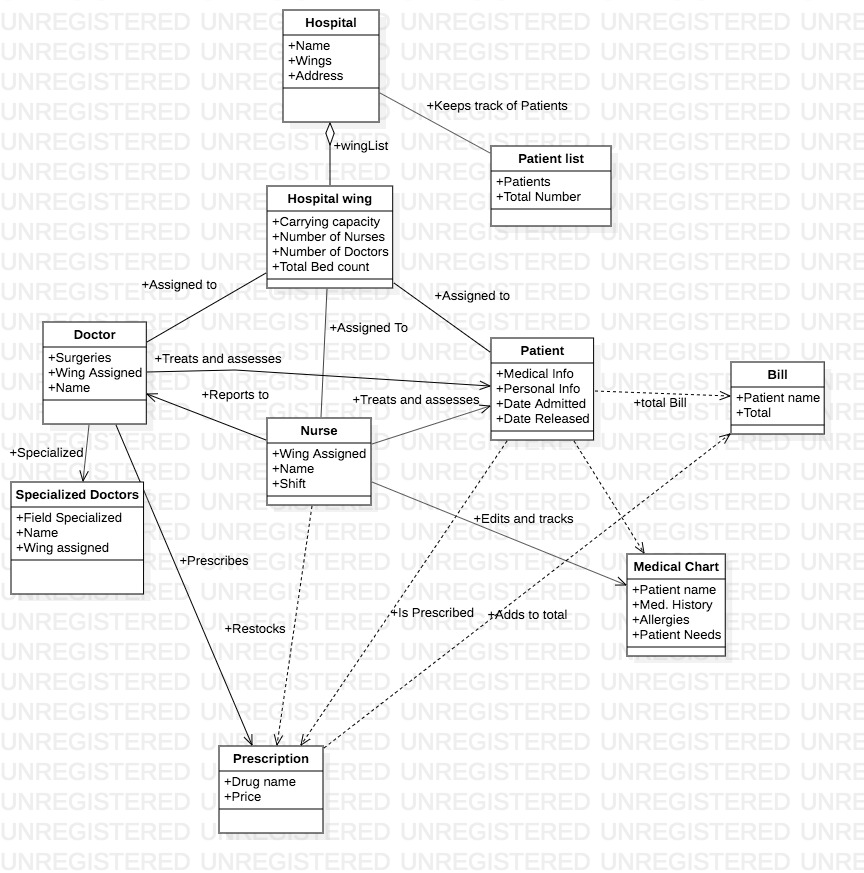
\includegraphics{OOAD Diagram}

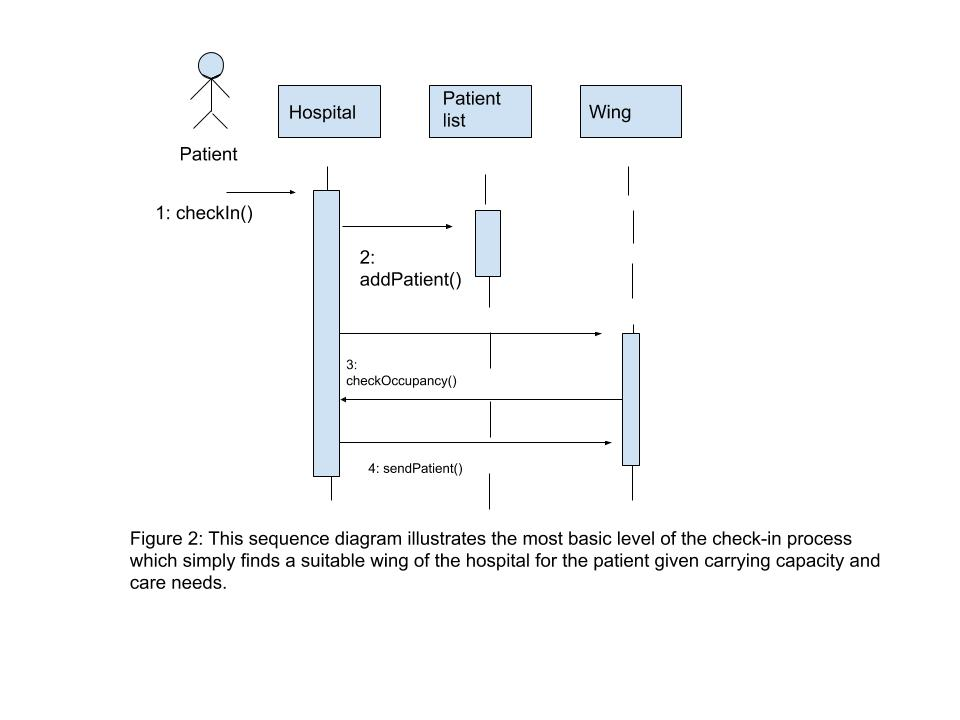
\includegraphics{Sequence Diagram 1}

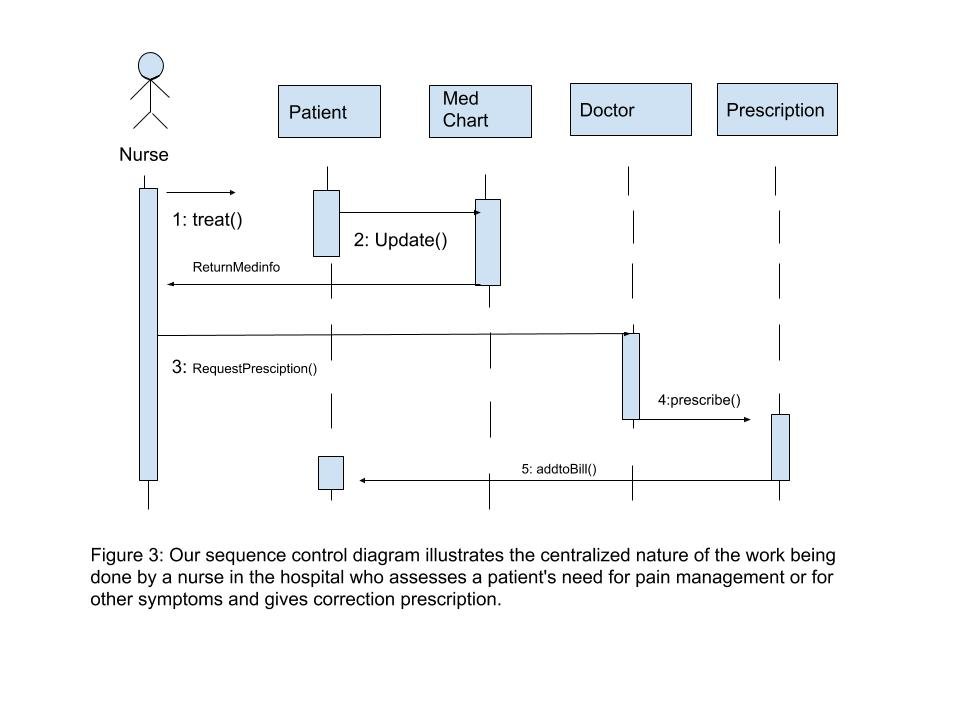
\includegraphics{Sequence diagarm 2}

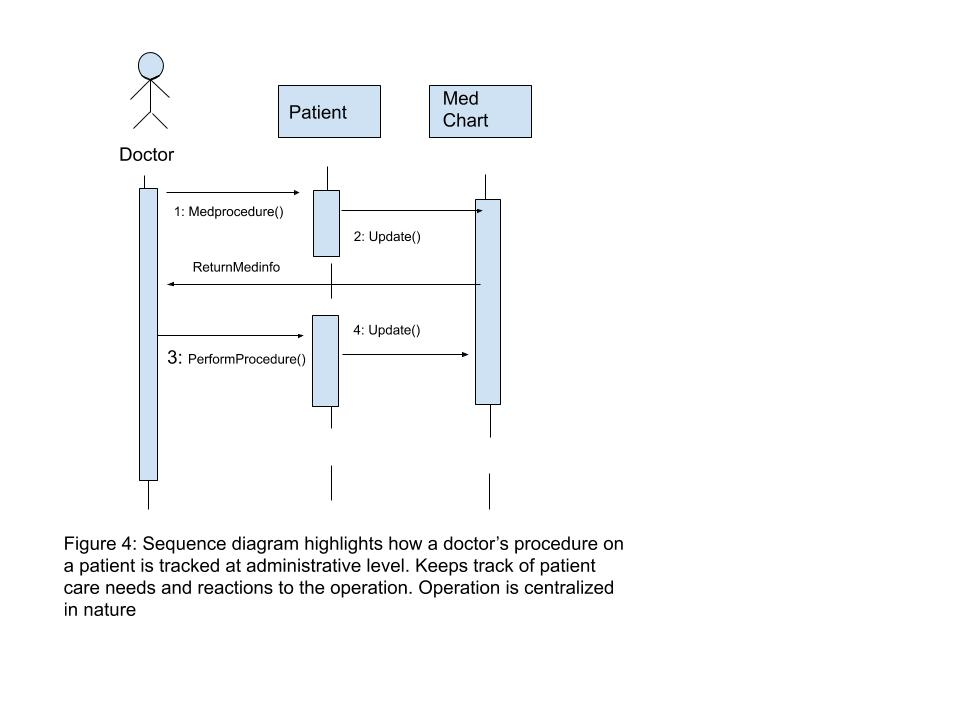
\includegraphics{Sequence 3}

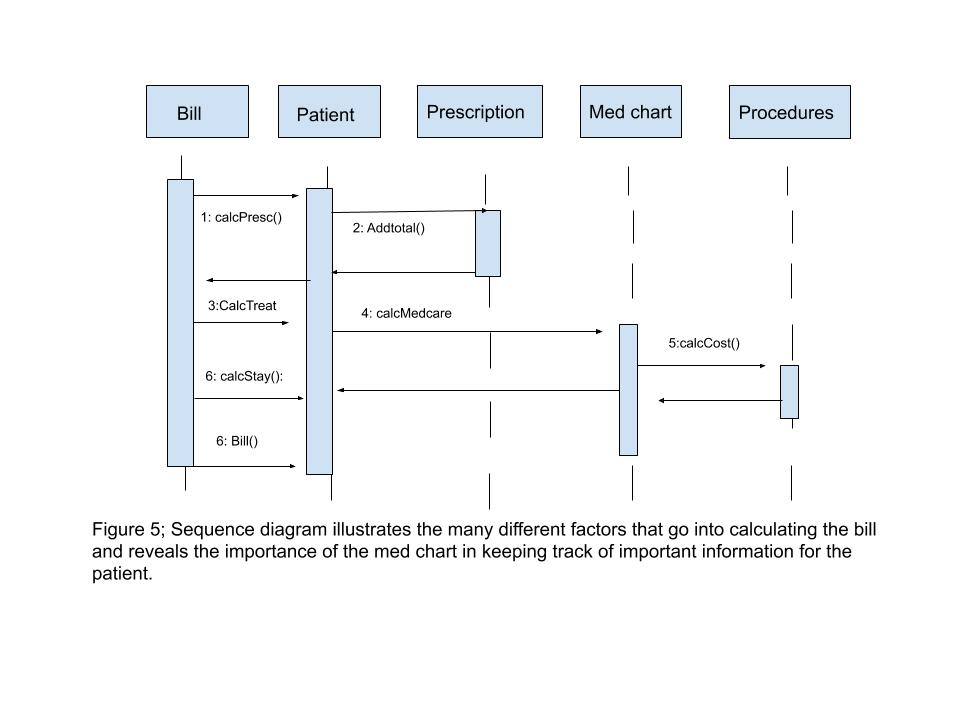
\includegraphics{Patient billing sequence 4}

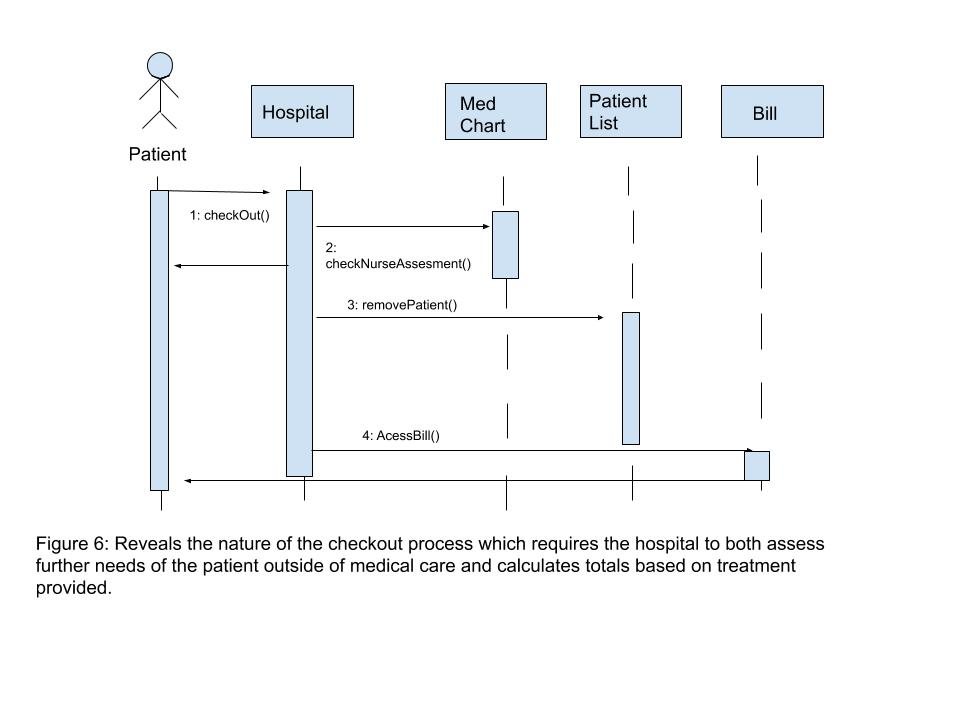
\includegraphics{Patient Checkout sequence 5}
    
\end{document}